\chapter{Introdução}
\label{cap:introducao}


\begin{flushright}
``Ordinary life is pretty complex stuff.''\\
(Harvey Pekar)
\end{flushright}

Os sistemas complexos compreendem um campo interdisciplinar da ciência que não possui uma definição exata. Este campo procura estudar numericamente um conjunto amplo de fenômenos não determinísticos, formados pela contribuição de um conjunto (geralmente grande) de componentes (muitas vezes simples) que, interagindo, estruturam-se de forma auto-organizada, gerando resultados inesperados, que não podem ser previstos pelos estudos estatísticos e/ou matemáticos tradicionais dos elementos formadores do sistema.

Na área dos estudos ambientais, os sistemas complexos possuem diversas aplicações: sistemas de transportes, redes de energia e comunicação, organizações sociais e econômicas, densidade e ocupação humana do espaço, dentre outas. Os estudos do clima ocupam um espaço de particular relevância na intercessão entre os estudos ambientais e os sistemas complexos. Em 2021 a Academia Real das Ciências da Suécia concedeu metade do Prêmio Nobel de Física para Syukuro Manabe e Klaus Hasselmann, cujos estudos apresentam modelos complexos para a análise do clima. Em particular apontam uma correlação entre as emissões de dióxido de carbono e as mudanças climáticas.

A aquisição, manipulação, gestão, armazenamento e criação de valor a partir de dados, através de ambientes computacionais, tem-se apresentado como um novo paradigma tecnológico. Um campo do conhecimento que recebeu a denominação de Ciência de Dados, conceito que envelopa alguns termos frequentemente associados à inovação científica, técnica e social como \emph{Big Data}, mineração de dados, \emph{Business Intelligence} internet das coisas, inteligência artificial e aprendizado de máquina(AM), dentre outros \cite[p. 12-13]{EMCdata2015}.

As séries temporais são definidas como um conjunto de observações (numéricas ou categóricas) ordenado no tempo.  Embora muitos dos dados que descrevem as dinâmicas espaciais podem ser registrados na forma de sérias temporais (abastecimento de água nas tubulações, consumo de energia elétrica nos imóveis, fluxos de pessoas e veículos pela cidade, casos de uma doença por dia, etc.), contudo as técnicas de medição de correlações, bem como a devida exploração destas para inferir novos conhecimentos, permanecem como perguntas abertas em muitas sub-áreas das ciências ambientais\cite{Bermudez-Edo2018}.


\section{Definição do problema}
\label{sec:problema}

Os fenômenos climáticos apresentam as características dos sistemas complexos. Um sistema integrado, envolvendo aspectos globais e as condicionantes planetárias, fatores locais de cobertura da terra, proximidade de corpos d'agua, regime de ventos, dentre outros. Em alguns casos, podendo citar o bioma dominante de um determinado lugar, o fator tanto influencia o clima quanto é influenciado por ele.

As inter-relações entre as diversas variáveis climáticas não podem ser facilmente correlacionadas em grande escala. É possível estabelecer relações entre certas medidas meteorológicas em uma determinada localidade, ainda que as relações entre essas não sejam necessariamente relações que podem ser transportadas para toda e qualquer localidade do planeta. Mas a possibilidade de estabelecer relações em rede entre as variáveis climáticas de diferentes localidades umas com as outras ainda é um problema aberto.

\section{Objetivos}
\label{sec:Objetivos}

O objetivo geral desta pesquisa é: investigar as correlações entre as variáveis climáticas através do coeficiente \dmc e utilizar o conhecimento destas correlações para alimentar um modelo preditivo do clima.

Como objetivos específico foram elencados:

\begin{enumerate}
    \label{enum:obj_espec}
    \item Implementar um algoritmo computacional geral para calcular o \dmc para qualquer número de séries temporais.
    \item Analisar um conjunto de dados climáticos contendo medições meteorológicas de todas as capitais brasileiras.
    \item Analisar um conjunto de dados meteorológicos sobre radiação solar com estações locadas em diversas partes do globo.
    \item Desenvolver e implementar um algoritmo de predição baseado em aprendizado de máquina e redes neurais artificias agregados com o coeficiente \dmc.
\end{enumerate}

\section{Importância da Pesquisa}
\label{sec:justificativa}

Um estudo mais amplo destas correlações pode levar a um entendimento maior dos fenômenos climáticos, e a modelos mais eficazes para previsão de aspectos do clima, podendo incluir os eventos climáticos extremos. 

A Organização das Nações Unidas (ONU) estabeleceu um conjunto de 17 objetivos em uma agenda que busca a melhoria das condições de vida no planeta e a mitigação de efeitos das mudanças climáticas (Agenda 2030). Denominados de Objetivos de desenvolvimento Sustentável (ODS). Pesquisas sobre o clima podem ser relacionadas diretamente com o ODS (13) Ação contra a mudança global do clima. Pode-se  encontrar importantes relações desta pesquisa com outros objetivos (2) Fome zero e agricultura sustentável, (6) Água potável e saneamento, (7) Energia limpa e acessível, (11) Cidades e comunidades sustentáveis, (14) Vida na água, (15) Vida na terra e, a difusão do conhecimento gerado nesta pesquisa pode levar a (17) Parceria e meios de implementação.



% \section{Limites e Limitações}
% \label{sec:limites}

\section{Questões e Hipóteses}
\label{sec:questoes}

Esta proposta foi baseada em duas premissas:

\begin{enumerate}
    \label{enum:premissas}
    \item Os fenômenos climáticos estão relacionados de forma complexa. Por exemplo: massas de ar percorrem distâncias na atmosfera e influenciam uma série de variáveis climáticas nas localidades por onde passam, mas que também são influenciadas, em seu percurso ou sua dissolução pelas mesmas variáveis.
    \item O \dmc, pelas características de análise do método, pode ajudar a entender estas correlações.
\end{enumerate}

Partindo destas premissas, procuramos responder duas perguntas basilares:

\begin{enumerate}
    \label{enum:quest}

    \item É possível estabelecer e medir correlações entre aspectos climáticos de uma determinada localidade e um conjunto de outras localidades?

    \item Em caso de resposta positiva, seria possível utilizar essas correlações para melhorar modelos climáticos preditivos?
\end{enumerate}

Para orientar o trabalho, duas hipóteses foram formuladas:

\begin{enumerate}
    \item Um método baseado no \dmc~seria um ferramental importante no estudo de correlações de variáveis climáticas envolvendo um grande número de localidades.
	\item É possível criar uma modelo preditivo para séries temporais de aprendizado de Máquina eficiente baseado no \dmc.
\end{enumerate}

\section{Aspectos Metodológicos}
\label{sec:metodologia}


\subsection{implementação do \dmc para um número qualquer de Variáveis independentes}

Embora esteja matematicamente definido, o \dmc~utiliza a inversão de matrizes no cálculo do coeficiente múltiplo. Este cálculo envolve o determinante da matriz e pode ser computacionalmente muito custoso.

A generalização proposta é a implementação de um algoritmo eficiente para o calculo do \dmc. A ideia é que este algoritmo seja publicado como um programa e um artigo sobre este programa pode ser submetido ao periódico \emph{Software X}, que tem um foco em publicações sobre programas científicos livres. Caso se entenda que o produto deste trabalho tem potencial para publicação em uma revista de maior fator de impacto, a mudança será feita.

Esta implementação é necessária para possibilitar a criação de um algoritmo de AM baseado no \dmc, visto que os estudos de ML baseiam-se na busca por padrões em um conjunto de atributos que costuma ser maior do que 1. Em seguida abordaremos o problema da criação do algoritmo. 

\subsection{Validação do modelo de AM}
\label{ssec:vlalid}
A validação do modelo de AM está representado na Figura~\ref{fig:fluxoGrimm}, baseada no diagrama de modelagem de Grimm e Railsback, um fluxograma circular que procura representar o trabalho de modelagem. Cada um dos nós deste fluxograma representa uma etapa do trabalho de modelagem.

Os nós da Pergunta~(1) e Hipótese~(2) estão descritos na Seção~\ref{quesHip} do Capitulo~\ref{intro} deste projeto. Os padrões esperados~(3) são os padrões de um algoritmo de AM: que após o treinamento, caso não aconteça um sobre-ajuste~(\emph{overfitting}), o modelo seja capaz de generalizar a informação obtida através da busca por padrões para as aplicações pretendidas.

\begin{figure}[!htb]
	\centering
	\caption{Diagrama de Grimm e Railsback}
	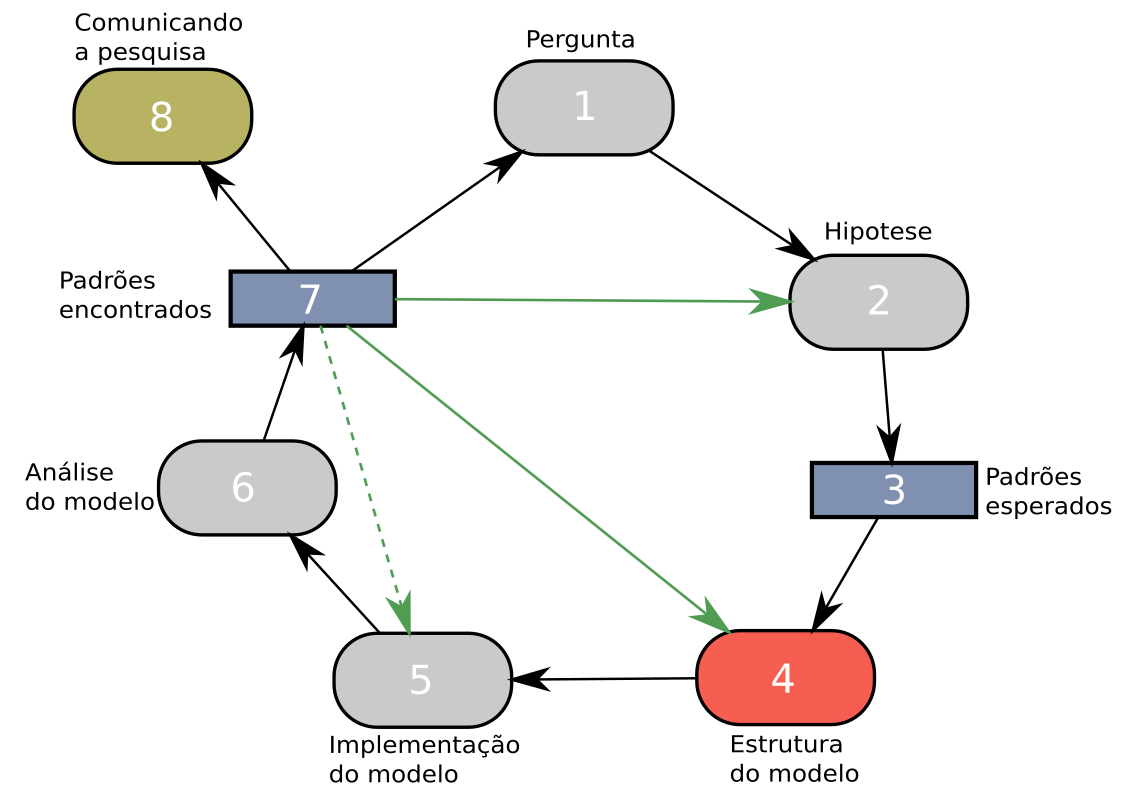
\includegraphics[width=.8\textwidth]{../Figures/intro/Ciclo_Grimm.png}
	\\{\footnotesize Fonte: Elaborada Pelo Autor}
	\label{fig:fluxoGrimm}
\end{figure}


O nó Estrutura do modelo~(4) representa um dos maiores desafios da tese: o de validar uma nova estrutura de modelos. Ao invés de buscar uma ferramenta de modelagem conhecida, pretende-se buscar, dentre as ferramentas conhecidas, aspectos que possam ser aproveitados na formatação de uma estratégia de AM baseada nas ferramentas também conhecidas do \pdcca~e \dmc.

A partir destas suposições, um modelo é implementado~(5) e será trainado e validado de acordo com os critérios de validação de um algoritmo de ML (separação dos dados em treinamento, validação e testes. Montagem da matriz de confusão, etc). O modelo será analisado(6) para verificar se ele repete os padrões esperados de um algoritmo de AM. A linha tracejada que parte do nó 7 para o nó 5 não existe no diagrama de Grimm e Railsback original, mas faz parte da rotina de ajustes de um modelo de AM. Caso se chegue a conclusão que o ajuste não é possível, retorna-se ao nó 4 e se reorganiza as bases utilizadas para criar o modelo. Caso se chegue a conclusão que nenhum ajuste é possível, refaz-se as hipóteses e/ou as perguntas norteadoras. 


\section{Organização da Tese}
\label{sec:organizacao}

A tese será formada pelos seguintes capítulos:
\begin{enumerate}
	\item Introdução
	\item Referencial teórico
	\item Metodologia
	\item Análise dos dados meteorológicos pelo \dmc
	\item Características e validação do modelo de AM proposto
	\item Tratamento dos dados de mobilidade urbana
	\item Aplicação do modelo proposto na análise da mobilidade urbana
	\item Conclusões
\end{enumerate}